%\documentclass[a4paper,11pt,bibtotoc,noliststotoc]{scrbook}
\documentclass[a4paper,11pt,titlepage,halfparskip,cleardoubleempty]{scrbook}
% -- Funcionalidades extras para las tablas
\usepackage{array}
\usepackage{multirow}
\usepackage{supertabular}
\usepackage{tabularx}
\usepackage{multirow}
\usepackage{dcolumn}
\usepackage{longtable}
% Codificación
\usepackage[spanish]{babel}
\usepackage[utf8x]{inputenc}

% Fuentes
\usepackage{lmodern}
\usepackage[T1]{fontenc}
\usepackage{textcomp}
\usepackage{colortbl}
% Formato de página
%\usepackage[ilines]{scrpage2}

% Otros paquetes
\usepackage{listings}
\usepackage{tabularx}
\usepackage{array}
\usepackage{xspace}
\usepackage{varioref}
\usepackage{microtype}
\usepackage{graphicx}
\usepackage[absolute]{textpos}
%\usepackage[rflt]{floatflt}
% Estilo para código:
\usepackage{color}
\definecolor{gray97}{gray}{.97}
\definecolor{gray75}{gray}{.75}
\definecolor{gray45}{gray}{.45}
\lstnewenvironment{listing}[1][]
   {\lstset{#1}\pagebreak[0]}{\pagebreak[0]}
\lstset{ frame=Ltb,
     framerule=0pt,
     aboveskip=0.5cm,
     framextopmargin=3pt,
     framexbottommargin=3pt,
     framexleftmargin=0.4cm,
     framesep=0pt,
     rulesep=.4pt,
     backgroundcolor=\color{gray97},
     rulesepcolor=\color{black},
     %
     stringstyle=\ttfamily,
     showstringspaces = false,
     basicstyle=\small\ttfamily,
     commentstyle=\color{blue},
     keywordstyle=\bfseries,
     %
     numbers=left,
     numbersep=15pt,
     numberstyle=\tiny,
     numberfirstline = false,
     breaklines=true,
   }
\lstdefinestyle{C++}
   {language=C++,
   }
% hyperref casi siempre es mejor cargarlo al final
\usepackage[colorlinks,citecolor=blue]{hyperref}

%\setheadsepline{.4pt}
\usepackage[left=2.5cm,top=3.5cm,right=2.5cm,bottom=3.5cm]{geometry}

\subject{Universidad de Cádiz \\ Programación en Entornos Cliente-Servidor\\ Curso 2011/2012}
\title{FreeMicroChat: Chat sencillo en C++}
\author{Aarón Bueno Villares\\Juan Antonio Tejero Fernández\\Inmaculada Labrador del Río}
\date{\today}

\makeatletter
\hypersetup{
  pdftitle={Documentación Chat en C++},
  pdfsubject={Programación en Entornos Cliente-Servidor 11/12},
  pdfauthor={Aarón Bueno Villares\\Juan Antonio Tejero Fernández\\Inmaculada Labrador del Río},
  pdfkeywords={pecs, cliente, servidor, chat, c++}
}
\makeatother

\newcommand{\cellcenter}[1]{\multicolumn{1}{c}{#1}}
\newcommand{\thead}[1]{\textbf{\emph{#1}}}
\newcommand{\espaciocambios}{\rule{0cm}{1.5cm}\xspace}
\setlength{\extrarowheight}{4pt}

\begin{document}
\newcommand{\reduce}{\fontsize{10}{11}\selectfont}
% Portada
\begin{titlepage}
%\includegraphics[scale=0.4]{Imagenes/logo-uca.png}
  \maketitle
%\includegraphics[width=5cm]{Imagenes/logo-uca.png}
\end{titlepage}

\frontmatter
\pagestyle{empty}

\tableofcontents
\listoffigures
%\listoftables


\mainmatter
%\pagestyle{scrheadings}
%%%%%%%%%%%%%%%%%%%%%% Capitulo 1: %%%%%%%%%%%%%%%%%%%%%%%%%%%%%
\chapter{Introducción}
\section{Motivación, por qué un chat}

Consideramos que sería interesante investigar como se trabaja con
sockets con C++, que es otro de los lenguajes más usados del mundo,
junto con Python o Java. El hecho de elegir un chat multiusuario como
hilo conductor de esta ``investigación'' vino motivada, sobre todo,
por su sencillez conceptual. No se pretendía crear algo útil ni con
fin de uso práctico, sino como muestra de ejemplo de cómo programar
son sockets en C++, así que la idea de un chat era suficiente para
cumplir con este propósito.


\section{Ideas fundamentales}
Hay dos ideas/pilares fundamentales en las que se basa nuestro chat:\\
\begin{itemize}
\item Asincronía:  Según la RAE; falta de coincidencia temporal en los hechos.
\item Delegación de funciones en el sistema operativo; conexión y recepción/envío de mensajes.
\end{itemize}



   En el servidor, todo es asíncrono. Es significa que las tareas de conexión/envío/recibo de mensajes se ''mandan'' al sistema operativo y el programa principal sigue trabajando. Será el sistema operativo quien se encargue de enviar y recibir los mensajes así como de establecer la conexíon con el servidor. Cuando finaliza alguna de estas acciones, el sistema operativo lo indica diparando un evento. Para estas llamadas asíncronas, se necesita, por tanto, una función a la que llamar cuando se dispare dicho evento y que tomen el control de la ejecución. Esta función recibe el nombre de 'callback'.

  \begin{figure} [h]
  \centering
   %\includegraphics[scale=0.35,angle=90]{Imagenes/WBS.png}
  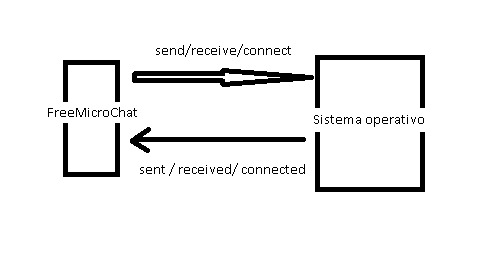
\includegraphics[width=200pt]{img/Callbacks-funct.png}
  \caption{Delegacion y Callback}
  %\label{fig:WSB_3.0}
  \end{figure}

\subsection{Asincronía y chats}

Toda conversación de chat es asíncrona, pues no se sabe cuándo llegarán mensajes por parte de otro usuario. Es por eso que el chat que debíamos crear debía cumplir esta característica.

\subsection{Asincronía en FreeMicroChat}

Para conseguir esa asincronía debíamos buscar una librería robusta y fiable que fuese capaz de trabajar sin problemas con este tipo de programas. Esa librería es Boost::Asio.


\subsection{Qué es Boost}
Boost, es un proyecto/repositorio de creación de librerías C++. Estas librerías C++ son libres (Boost Software License) y están revisadas por profesionales. Además, éstas trabajan ''bien'' con la librería estándar de C++. Boost cuenta con unas 40 librerías en total, cada con un 'marco' de trabajo.

\subsection{Por qué Boost}
Estas son algunas de las razones por las que nos decantamos por Boost:
\begin{itemize}
\item Cuenta con una documentación amplísima en la que se incluyen ejemplos.
\item Está ''viva'', es decir que continuamente se van añadiendo nuevas librerías, ejemplos, etc... al contar con una amplia comunidad que la mantiene.
\item Muy utilizada por los desarrolladores profesionales de aplicaciones de este tipo,  empresas y herramientas como: \textit{Adobe Software Libraries},   \textit{LyX Document Editor}  o  \textit{The C++/Tk Library}.
\item Diez de las librerías de Boost están incluídas en librería estándar de C++ TR1, y se pretende que en el futuro estén incluídas todas sus librerías.
\end{itemize}


\subsection{Qué es Boost::Asio}

Boost::Asio es una librería C++ multi-plataforma para redes y programación de E/S a bajo nivel que proporciona desarrolladores, con un modelo asíncrono consistente usando un enfoque de C++ moderno. En definitiva, es la librería de Boost, para la programación de redes (entre otras cosas).

\section{Lógica de funcionamiento}
\subsection{Servidor}
  El servidor maneja varios clientes, y los comunica entre sí. Cuando se conecta   un cliente, éste tiene que enviarle su nick. Una vez que el servidor ha recibido   dicho nick, el servidor le envía al nuevo cliente la lista de contactos.\\

  El servidor entonces 'escucha' a dicho cliente. Cada vez que dicho cliente le envía un  mensaje, éste contendrá a su destinatario. A continuación el servidor envía el mensaje a dicho  destinatario. A su vez, cada vez que un nuevo cliente se conecta o se desconecta, envía  la lista de contactos actualizada a cada uno de sus clientes actualmente conectados.\\

\subsection{Cliente}
  El cliente se conecta a un solo servidor. Cuando se conecta le envía su nick, y luego recibe la lista de contactos. Cada vez que quiere enviar un mensaje, indica quién es el destinatario. Y cuando el cliente recibe un mensaje del servidor, también recibe  quién es el emisor.



%%%%%%%%%%%%%%%%%%%%%% Capitulo 2: %%%%%%%%%%%%%%%%%%%%%%%%%%%%%
\chapter{Referencias}
\begin{itemize}
\item \htmladdnormallink{Documentación oficial}{ http://www.boost.org/doc/libs/1_46_1/doc/html/boost_asio.html}
\item \htmladdnormallink{Manual de inicio}{http://www.gamedev.net/blog/950/entry-2249317-a-guide-to-getting-started-with-boostasio?pg=1}

\end{itemize}

%%%%%%%%%%%%%%%%%%%%%% Capitulo 3: %%%%%%%%%%%%%%%%%%%%%%%%%%%%%
\chapter{Boost::Asio}
%%%%%%%%%%%%%%%%%%% Apartado 3.1:
\section{Clases y funciones}


\begin{lstlisting}[style=C++]
Boost::Asio::io_service:
\end{lstlisting}

Clase de \textit{Boost::Asio} que incluye facilidades para programadores que desarrollan servicios asíncronos personalizados.\\

\begin{lstlisting}[style=C++]
boost::asio::io_service::run():
\end{lstlisting}
Función que ejecuta (el evento de bucle procesamiento de) un objeto tipo  \textit{io\_service}. Bloquea la finalización del programa mientras haya operaciones pendientes sin finalizar. Por tanto, se debe llamar a  \textit{io\_service::run()} inmediatamente después de ejecutar la primera operación asíncrona.\\


Secuencia de eventos en operaciones asíncronas.
\begin{enumerate}
\item Nuestro programa inicia una operación de conexión llamando a un objeto tipo I/O (por ejemplo, un  \textit{socket})
\item El objeto de I/O prolonga la petición hasta un objeto tipo  \textit{io\_service}.
\item   \textit{io\_service} indica al sistema operativo que él debería comenzar una conexión asíncrona.
\item El sistema operativo indica que la operación de conexión ha sido completada, colocando el resultado de esta operación en una cola.
\item El programa debe realizar una llamada a  \textit{io\_service::run()} con el objetivo de que dentro de  \textit{io\_service::run()} se recupere el resultado desde la cola.
\item 6. El flujo de ejecución pasa a la función de  \textit{callback} que deba ejecutarse.
\end{enumerate}

Este proceso lo puede observar gráficamente en las imágenes  \ref{img:sec1} y \ref{img:sec2}.


  \begin{figure}[h!]

  \centering
     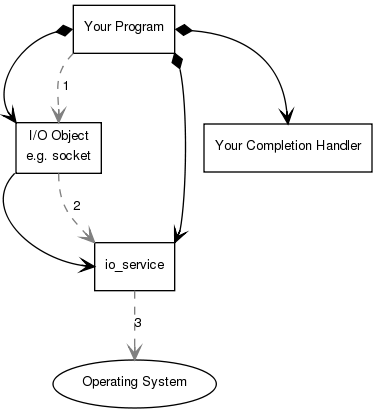
\includegraphics[width=165pt]{img/async_op1.png}
    \caption{Eventos en operaciones asíncronas - Fase 1}
\label{img:sec1}
  \end{figure}





  \begin{figure}[h!]
  \centering
     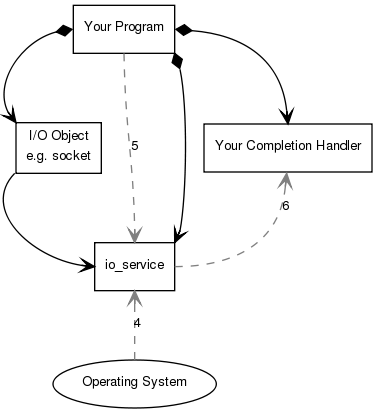
\includegraphics[width=165pt]{img/async_op2.png}
    \caption{Eventos en operaciones asíncronas - Fase 2}
\label{img:sec2}
  \end{figure}




\section{Envío de mensajes a través de la red: Serialización}

Cuando enviamos datos a través de la red, éstos no pueden ir ''de cualquier forma'', es decir, si queremos enviar por ejemplo un objeto de un tipo  \textit{ClaseA} no podemos enviarlo directamente.
\begin{enumerate}
\item Antes se debe realizar una transformación de  \textit{ClaseA::objeto} a  \textit{texto}.
\item A continuación enviamos el dato.
\item Una vez en el destino se debe deshacer esta transformación y podremos hacer uso de ese  \textit{ClaseA::objeto}.
\end{enumerate}

Todo este proceso de tranformación entre tipos lo realizamos con  \textit{Python} a través de  \textit{JSON} y en C++ se realiza a través de la serialización.

\subsection{Serializacion en FreeMicroChat}
Un ejemplo de serialización es el siguiente, en el que se serializa y des-serializa un mensaje:
\begin{lstlisting}[style=C++]

Message::serialize()
    std::ostringstream oss;
    text_oarchive ar(oss);/* serializacon del mensaje*/
    ar << *this;

Message::Message(... buffer)
{
    istream is(&(*buffer));
    text_iarchive ar(is); /* des-serializacion del mensaje */
    ar >> *this;
\end{lstlisting}

%%%%%%%%%%%%%%%%%%%%%% Capitulo 3: %%%%%%%%%%%%%%%%%%%%%%%%%%%%%
\chapter{Implementacion}
\section{Arquitectura}
En la imagen  \ref{img:arq} se puede observar qué clases posee el sistema y cómo está relacionadas las unas con las otras.


\begin{figure}[h!]
\centering
     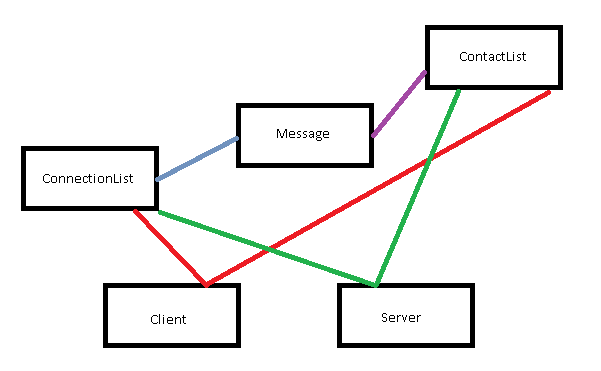
\includegraphics[width=250pt]{img/Arquitectura.png}
    \caption{Clases y sus relaciones}
\label{img:arq}
  \end{figure}





  \section{Diseño general del código}

  Existen las clases \textit{Server, Client, Message, ContactList, ConnectionList}. \\
Por otro lado,  todos estos ficheros contiene la cabecera Headers.hpp. Debido a que boost es un poco
  ''engorroso'', en esta cabecera están todas las definiciones y \textit{typedefs} que se necesitarán
  a lo largo del código.\\

\subsection{ConnectionList}
  Las clase \textit{ConnectionList} es una interfaz entre \textit{Server/Client} y los \textit{sockets} de
  \textit{boost::asio}. De esta forma, cuando se quieren enviar o recibir mensajes, \textit{Server/Client}
  interactúan con \textit{ConnectionList}, que tiene una interfaz bastante más amigable  que \textit{asio}.

  \subsection{ContactList y Message}
  \textit{ContactList} es una lista de \textit{nicks}. Cada \textit{nick} viene señalado por un identificador
  \textit{unsigned}. \textit{Server} y \textit{Client} solo se envían dichos identificadores, mientras que
  el usuario ve en su pantalla solamente el \textit{nick} asociado.

 \textit{Message} es una clase que tiene tres atributos:
\begin{itemize}
     \item MessageType:
\begin{itemize}
        \item MSG\_NULL para indicar mensaje nulo.

                    \item MSG\_EOF  para indicar fin de conexión.
                    \item MSG\_CONTACT\_LIST para indicar que se está enviando la lista
                             de contactos (solo lo envía Server).
                    \item MSG\_NICK para indicar que se envía un nick (solo lo envía Client).
            \end{itemize}
     \item Message: El contenido en sí.
     \item Target: Identificador del destinatario cuando se envía, y el emisor cuando se
               recibe.
\end{itemize}
   Los mensajes se envía serializandose (función \textit{Message::serialized()}), y se deserializan
   con uno de sus constructores.
  Para enviar la lista de contactos, se envía un mensaje
   de tipo MSG\_CONTACT\_LIST cuyo mensaje es la serialización de la lista de contactos:
   \textit{ContactList::serialize()}. La lista de contactos se deserializa con el método
   \textit{ContactList::deserialize()}.\\

   La clase \textit{ContactList} tiene dos ''grupos'' de métodos. El primero es relacionado con lo
   que he decido en llamada: \textit{PhantomContact}. Son contactos que se han conectado al
   servidor pero todavía no han enviado su \textit{nick}. Cuando el \textit{nick} ha sido recibido,
   se ''registra'' dicho contacto fantasma en la verdadera lista de contactos, con la
   función \textit{ContactList::checkinPhantomContact}, que recibe el identificador del contacto.
\\
   \textit{ConnectionList}
   Esta clase es una lista de \textit{sockets} y \textit{bufferes}. Es decir, para cada identificador
   definido en la lista de contactos, se tiene un \textit{socket} y dos \textit{bufferes}: uno para
   los datos recibidos, y otro para enviar datos.\\

   Esta clase es una interfaz por encima de \textit{boost::asio}. Es decir, automatiza el
   envío y recepción de datos:
\begin{itemize}
\item Recibir datos: para recibir datos, la función \textit{boost::asio::asyn\_write(...)}
                     necesita un buffer en donde escribir. Este buffer será el
                     buffer de recepción nombrado más arriba. Cuando éstos
                     éstan listos, ConnectionList encapsula los datos recibidos en
                     el \textit{buffer} en un \textit{Message}, que será devuelto al \textit{Server/Client} (a quién corresponda).
\item Enviar datos: Análogo a recibir datos. Una vez recibido el dato, ConnectionList
                    reenvia el Message enviado a \textit{Server/Cllient} (a quién corresponda).
                    Si hay algún error (en particular, si la comunicación se ha cerrado),
                    se crea un mensaje \textit{MSG\_EOF} que se devuelve al \textit{Server/Client} en vez
                    del mensaje original (es de observar que mensajes del tipo \textit{MSG\_EOF}
                    nunca se envían a través del socket, solamente en dirección
                    \textit{ConnectionList->Server/Client}). Si hay un error recibiendo datos,
                    se procede como aquí: enviando un \textit{MSG\_EOF} a \textit{Server/Client}.
\end{itemize}
   Si \textit{Server/Client} recibe un mensaje de tipo \textit{MSG\_EOF} por parte de \textit{ConnectionList},
   le dice luego a \textit{ConnectionList} que elimine la conexión (\textit{ConnectionList::deleteConection}),
   lo que implica también cerrar el \textit{socket}. En caso del \textit{Client}, como solamente tiene
   una conexión (con el \textit{Server}), cerrar la conexión implica abandonar el programa.\\

\subsection{Server}
   El funcionamiento de \textit{Server}, aunque abstraido de la ''sintaxis'' y requerimientos
   de \textit{boost::asio} gracias a la clase \textit{ConnectionList}, sí que tienen en común su forma
   de trabajar, ya que la librería así lo impone.

   Como se comentaba al principio, en el servidor todo es asíncrono y que de las tareas de conexión/envío/recibo de mensajes se ocupa sistema operativo de forma que el programa principal sigue trabajando. Una vez que el sistema operativo finalice el flujo de ejecución pasará a una función de \textit{callback}. Esa función será ejecutada
   en cualquiera de los hilos del programa que estén ejecutando a la función \textit{io\_service->run()}.

   Esta función es una función que no acaba hasta que ''no haya más trabajo que hacer''.
   Es decir, mientras que haya eventos/\textit{callbacks} por procesar, la función no ''retornará'', y por
   lo tanto mantendrá al hilo ocupado.

   \textit{Server} solo tiene un único hilo, el propio hilo del programa, así que él es el que ejecuta
   a la función \textit{run()}. Justo antes de hacerlo, el servidor inicia al \textit{loop} de conexiones: \textit{\_connectionControl()}.
   Esto llama a \textit{async\_connect()} con \textit{Server::\_newClient()} como \textit{callback}. Justo después de la llamada
   a \textit{async\_connect()} es cuando se ejecuta \textit{run()}, que se mantendrá latente hasta que no se ejecute dicho
   \textit{callback}, es decir, hasta que no llegue un nuevo cliente. Cuando llegue, la función \textit{\_newClient()}
   se ejecutará en el hilo actual (ya que \textit{run()} se llamó aquí).

   A partir de aquí, todas las llamadas asíncronas se hacen a través de \textit{ConnectionList}.
   La secuencia de callbacks completa es la siguiente:\\
 \textit{    \_connectionControl()} -> \textit{\_newClient()} -> \textit{\_getNick()} -> \textit{\_newMsg()} -> \textit{\_newMsg()}\\
 \textit{    \_connectionControl()} -> \textit{\_connectionControl()}

   De esta forma, cada vez que llega una conexión, se espera a por otra, mientras se espera
   recibir el \textit{nick}, y luego sucesivos mensajes. Esto crea una ''linea'' de \textit{callbacks} por cada
   nuevo cliente llegado. De esta forma, la función \textit{run()} al menos tiene siempre un \textit{callback}
   pendiente: el de la llegada de un nuevo cliente, así que la función nunca ''retornará''.
   La única forma de detener al cliente es cerrandolo forzosamente desde fuera.

   \subsection{Client}
   Una vez comprendido como funciona el servidor, el cliente es análogo, con la diferencia de que,
   como solamente hay una conexión (al \textit{Server}), la conexión es síncrona (es decir,
   hasta que no se conecte no continúa).\\

   La secuencia de callbacks después de la conexión es la siguiente:\\
     \textit{\_talkLoop()} -> \textit{\_sendedNick()}\\
     \textit{\_talkLoop()} -> \textit{\_recvContactList()} ->\textit{\_newMsg()} -> \textit{\_newMsg()}

   Cuando se recibe la lista de contactos, se ejecuta un nuevo hilo
   con la función \textit{\_readMsg()}, que se encarga de leer los mensajes escritos
   por el usuario para enviárselos al servidor. La secuencia de \textit{callbacks}
   es:\\
     \textit{\_readMsg()} -> \textit{\_sendedMsg()}\\
     \textit{\_readMsg()} -> \textit{\_readMsg()}\\

   Cuando el cliente recibe algún mensaje del tipo \textit{MSG\_EOF}, significa que el servidor se ha caido
   o ha cerrado la conexión, momento en el que \textit{Client} llama a la función \textit{exit()} y se termina
   el programa.

%%%%%%%%%%%%%%%%%%%%%% Capitulo 4: %%%%%%%%%%%%%%%%%%%%%%%%%%%%%
\chapter{Manuales}
\section{Instalación}

FreeMicroChat ha sido desarrollado y ejecutado bajo el siguiente entorno de trabajo:
\begin{itemize}
\item Versión de librería: Boost::Asio 1\_46\_1. Descargar desde: \htmladdnormallink{aquí}{ http://sourceforge.net/projects/boost/files/boost/1.46.1/}
\item Colocar la carpeta con las librerías en: /usr/local
\item Sistema Operativo: Ubuntu 11.10
\item Librerías: libboost-thread1.46-dev libboost-system1.46-dev libasio-dev. Instalar desde gestor de paquetes.
\end{itemize}


%%%%%%%%%%%%%%%%%%%%%% Capitulo 4: %%%%%%%%%%%%%%%%%%%%%%%%%%%%%
\section{Manual de usuario}

  Cuando se ejecuta este programa, puede ejecutarse como cliente o como servidor.\\

  Como servidor:
\begin{lstlisting}[style=C++]
    ./FreeMicroChat server port
\end{lstlisting}

Como cliente:
\begin{lstlisting}[style=C++]
      ./FreeMicroChat client server_ip server_port user_nick
\end{lstlisting}
  Evidentemente, hay que ejecutar el servidor antes de ejecutar a cualquier cliente.

Cliente:\\

\begin{itemize}
\item  Usuarios conectados: Si el cliente quiere ver la lista de contactos, puede escribir \textit{\$} y luego la tecla \textit{Enter}. Aparecerá entonces la lista de todos los usuarios conectados.
  lo que verá es un \textit{prompt} tal que así:\\
\textit{Nick\$>}.\\
\item Seleccionar un destinatario:
Si escribe el nombre de otro cliente, el \textit{prompt} cambia de la siguiente forma:\\
\textit{Nick->NickDestino\$>}
\item Mandar un mensaje: Una vez seleccionado el destinatario todo lo que escriba el usuario será dirigido a \textit{NickDestino}. Pulsando \textit{Enter} se enviará el mensaje.\\
\item Mensajes recibidos: Cada vez que el usuario pulsa \textit{Enter}, aparecerá en su pantalla todos los
  mensajes recibidos (en caso de que haya algunos). Estos mensajes tendrán el formato \textit{NickEmisor->Nick\$>Mensaje}.\\ De esta forma se indica siempre la dirección del mensaje.
\item Para salir, tendrá que introducir \textit{exit}.
\end{itemize}
%\begin{figure}[!h]
%  \centering
%\includegraphics[scale=0.35,angle=90]{Imagenes/WBS.png}
%  \includegraphics[scale=0.30]{Imagenes/WBS.png}
%  \caption{Diagrama WBS del proyecto}
%  \label{fig:WSB}
%\end{figure}


%\backmatter
%\bibliographystyle{hispa}
%\bibliographystyle{plain}
%\bibliography{bibliografia.bib}
%\label{cap:bibliografia}


\end{document}

%%% Local Variables:
%%% mode: latex
%%% TeX-master: t
%%% End:
